\documentclass[11pt,a4paper]{article}
\usepackage[utf8]{inputenc}
\usepackage[T1]{fontenc}
\usepackage[english]{babel}
\usepackage{amsmath}
\usepackage{amssymb}
\usepackage[margin=1.8cm]{geometry}
\usepackage{lmodern}
\usepackage{xcolor}
\usepackage{setspace}
\usepackage{tikz}
\usetikzlibrary{arrows.meta}
\pagestyle{empty}
\setlength{\parindent}{0pt}
\setlength{\parskip}{0.8em}
\linespread{1.15}

\tikzset{
  resistor/.style={
    draw,
    rectangle,
    minimum width=1.05cm,
    minimum height=0.38cm,
    inner sep=1pt,
    font=\small
  },
  terminal/.style={
    circle,
    fill=black,
    inner sep=1.5pt
  }
}

\newcommand{\answernote}[1]{%
\vfill
\noindent\textcolor{gray}{\rule{\linewidth}{0.4pt}}

{\small\textcolor{gray}{Correct answer: #1}}
}

\begin{document}

{\LARGE\textbf{Question 1}}

Two point charges are separated by a distance $r$, and the force between them has magnitude $F$.

The first charge is multiplied by $2$, the second charge is multiplied by $4$, and the distance between the charges is multiplied by $4$. The new magnitude of the Coulomb force is:

\vspace{0.5em}

{\large
\textbf{A.} $2F$

\textbf{B.} $\frac{1}{2}F$

\textbf{C.} $\frac{1}{4}F$

\textbf{D.} $8F$
}

\answernote{B}
\newpage

{\LARGE\textbf{Question 2}}

The electric potential on the $x$-axis is given by

\[
V(x)=12-3x^2
\]

where $x$ is measured in meters and $V$ in volts.

Using the relation $E_x=-\frac{dV}{dx}$, the electric field component $E_x$ at $x=2$ is:

\vspace{0.5em}

{\large
\textbf{A.} $-12\ \mathrm{V/m}$

\textbf{B.} $-6\ \mathrm{V/m}$

\textbf{C.} $6\ \mathrm{V/m}$

\textbf{D.} $12\ \mathrm{V/m}$
}

\answernote{D}
\newpage

{\LARGE\textbf{Question 3}}

A particle of mass

\[
m=0.01\ \mathrm{kg}
\]

and charge

\[
q=+2\ \mathrm{mC}
\]

moves in a uniform electric field

\[
\vec E=(0,50)\ \mathrm{N/C}
\]

with initial velocity

\[
\vec v(0)=(3,4)\ \mathrm{m/s}.
\]

The velocity after $t=2\ \mathrm{s}$ is:

\vspace{0.5em}

{\large
\textbf{A.} $(3,14)\ \mathrm{m/s}$

\textbf{B.} $(3,24)\ \mathrm{m/s}$

\textbf{C.} $(13,4)\ \mathrm{m/s}$

\textbf{D.} $(23,4)\ \mathrm{m/s}$
}

\answernote{B}
\newpage

{\LARGE\textbf{Question 4}}

A charged particle moves with velocity

\[
\vec v=(2,0,0)\ \mathrm{m/s}
\]

in a magnetic field

\[
\vec B=(0,0,3)\ \mathrm{T}
\]

For a positive charge $q=1\ \mathrm{C}$, the magnetic force is:

\vspace{0.5em}

{\large
\textbf{A.} $(0,-6,0)\ \mathrm{N}$

\textbf{B.} $(0,6,0)\ \mathrm{N}$

\textbf{C.} $(6,0,0)\ \mathrm{N}$

\textbf{D.} $(0,0,6)\ \mathrm{N}$
}

\answernote{A}
\newpage

{\LARGE\textbf{Question 5}}

The magnetic flux through a conducting loop changes in time according to

\[
\Phi(t)=3t^2-2t
\]

in SI units. Using Faraday's law with sign convention $\mathcal E=-\frac{d\Phi}{dt}$, the induced electromotive force at $t=1\ \mathrm{s}$ is:

\vspace{0.5em}

{\large
\textbf{A.} $-4\ \mathrm{V}$

\textbf{B.} $4\ \mathrm{V}$

\textbf{C.} $-1\ \mathrm{V}$

\textbf{D.} $1\ \mathrm{V}$
}

\answernote{A}
\newpage

{\LARGE\textbf{Question 6}}

In an RL circuit, after the power supply is removed but the circuit remains closed through the resistor, the current decreases according to

\[
I(t)=I_0 e^{-t/\tau},
\]

where the time constant is

\[
\tau=\frac{L}{R}.
\]

For

\[
L=2\ \mathrm{H}, \qquad R=4\ \Omega, \qquad I_0=3\ \mathrm{A},
\]

the current at $t=0.5\ \mathrm{s}$ is:

\vspace{0.5em}

{\large
\textbf{A.} $3e^{-1}\ \mathrm{A}$

\textbf{B.} $3e^{-2}\ \mathrm{A}$

\textbf{C.} $3e^{-1/2}\ \mathrm{A}$

\textbf{D.} $3e^{-4}\ \mathrm{A}$
}

\answernote{A}
\newpage

{\LARGE\textbf{Question 7}}

All resistors in the circuit below have resistance $1\ \Omega$.

\begin{center}
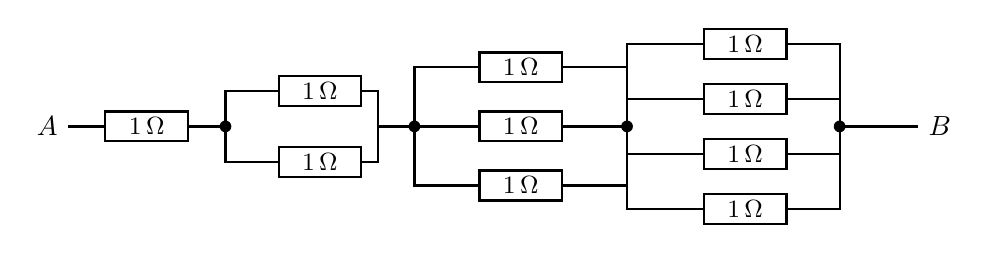
\begin{tikzpicture}[line width=0.8pt, x=1cm, y=1cm]
  \coordinate (A) at (0,0);
  \coordinate (P1) at (2.0,0);
  \coordinate (P2) at (4.4,0);
  \coordinate (P3) at (7.1,0);
  \coordinate (P4) at (9.8,0);
  \coordinate (B) at (10.8,0);

  \node[left] at (A) {$A$};
  \node[right] at (B) {$B$};

  \node[resistor] (R1) at (1.0,0) {$1\,\Omega$};
  \draw (A) -- (R1.west);
  \draw (R1.east) -- (P1);
  \node[terminal] at (P1) {};

  \node[resistor] (R2a) at (3.2,0.45) {$1\,\Omega$};
  \node[resistor] (R2b) at (3.2,-0.45) {$1\,\Omega$};
  \draw (P1) -- ++(0,0.45) -- (R2a.west);
  \draw (P1) -- ++(0,-0.45) -- (R2b.west);
  \draw (R2a.east) -- ++(0.2,0) -- ++(0,-0.45) -- (P2);
  \draw (R2b.east) -- ++(0.2,0) -- ++(0,0.45) -- (P2);
  \node[terminal] at (P2) {};

  \node[resistor] (R3a) at (5.75,0.75) {$1\,\Omega$};
  \node[resistor] (R3b) at (5.75,0) {$1\,\Omega$};
  \node[resistor] (R3c) at (5.75,-0.75) {$1\,\Omega$};
  \draw (P2) -- ++(0,0.75) -- (R3a.west);
  \draw (P2) -- (R3b.west);
  \draw (P2) -- ++(0,-0.75) -- (R3c.west);
  \draw (R3a.east) -| (P3);
  \draw (R3b.east) -- (P3);
  \draw (R3c.east) -| (P3);
  \node[terminal] at (P3) {};

  \node[resistor] (R4a) at (8.6,1.05) {$1\,\Omega$};
  \node[resistor] (R4b) at (8.6,0.35) {$1\,\Omega$};
  \node[resistor] (R4c) at (8.6,-0.35) {$1\,\Omega$};
  \node[resistor] (R4d) at (8.6,-1.05) {$1\,\Omega$};
  \draw (P3) -- ++(0,1.05) -- (R4a.west);
  \draw (P3) -- ++(0,0.35) -- (R4b.west);
  \draw (P3) -- ++(0,-0.35) -- (R4c.west);
  \draw (P3) -- ++(0,-1.05) -- (R4d.west);
  \draw (R4a.east) -| (P4);
  \draw (R4b.east) -| (P4);
  \draw (R4c.east) -| (P4);
  \draw (R4d.east) -| (P4);
  \draw (P4) -- (B);
  \node[terminal] at (P4) {};
\end{tikzpicture}
\end{center}

The equivalent resistance between points A and B is:

\vspace{0.5em}

{\large
\textbf{A.} $\left(1+\frac12+\frac13+\frac14\right)\ \Omega$

\textbf{B.} $\left(1+\frac13+\frac14+\frac15\right)\ \Omega$

\textbf{C.} $\frac{1}{1+2+3+4}\ \Omega$

\textbf{D.} $4\ \Omega$
}

\answernote{A}
\newpage

{\LARGE\textbf{Question 8}}

A capacitor $C$ is initially uncharged. At $t=0$, it is connected to a DC voltage source $U_0$ through a resistor $R$.

\begin{center}
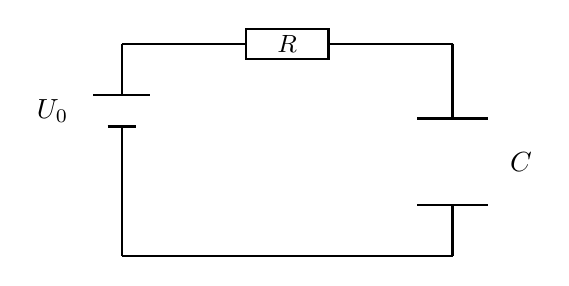
\begin{tikzpicture}[line width=0.8pt, x=1cm, y=1cm]
  \coordinate (TL) at (0,1.5);
  \coordinate (TR) at (4.2,1.5);
  \coordinate (BR) at (4.2,-1.2);
  \coordinate (BL) at (0,-1.2);

  \node[resistor] (R) at (2.1,1.5) {$R$};
  \draw (TL) -- (R.west);
  \draw (R.east) -- (TR);
  \draw (BR) -- (BL);
  \draw (TL) -- (0,0.85);
  \draw (0,0.45) -- (BL);
  \draw (-0.36,0.85) -- (0.36,0.85);
  \draw (-0.18,0.45) -- (0.18,0.45);
  \node[left] at (-0.55,0.65) {$U_0$};
  \draw (TR) -- (4.2,0.55);
  \draw (4.2,-0.55) -- (BR);
  \draw (3.75,0.55) -- (4.65,0.55);
  \draw (3.75,-0.55) -- (4.65,-0.55);
  \node[right] at (4.8,0) {$C$};
\end{tikzpicture}
\end{center}

The voltage across the capacitor is described by:

\vspace{0.5em}

{\large
\textbf{A.} $U_C(t)=U_0 e^{-t/(RC)}$

\textbf{B.} $U_C(t)=U_0 e^{-tR/C}$

\textbf{C.} $U_C(t)=U_0\left(1-e^{-t/(RC)}\right)$

\textbf{D.} $U_C(t)=U_0 e^{-RCt}$
}

\answernote{C}
\newpage

{\LARGE\textbf{Question 9}}

The circumference of the Earth was estimated in ancient Greece by comparing the angle of sunlight at two different locations. This measurement is usually attributed to:

\vspace{0.5em}

{\large
\textbf{A.} Aristotle

\textbf{B.} Archimedes

\textbf{C.} Eratosthenes

\textbf{D.} Ptolemy
}

\answernote{C}
\newpage

{\LARGE\textbf{Question 10}}

When determining $g$ from the period of a simple pendulum, it is better to measure the time of 10 oscillations instead of only one oscillation because:

\vspace{0.5em}

{\large
\textbf{A.} the pendulum has a different period during the first oscillation

\textbf{B.} the relative effect of reaction-time error is reduced

\textbf{C.} the formula for $g$ works only for 10 oscillations

\textbf{D.} measuring 10 oscillations eliminates all systematic errors
}

\answernote{B}

\end{document}
